\documentclass[12pt,a4paper,oneside]{report}
\usepackage{fontspec}
\setmainfont{Noto Sans CJK SC}
\setsansfont{Noto Sans CJK SC}
\setmonofont{DejaVu Sans Mono}
\XeTeXlinebreaklocale "zh"
\XeTeXlinebreakskip = 0pt plus 1pt
\usepackage[margin=2.55cm]{geometry}
\usepackage{booktabs,longtable,array,tabularx,multirow}
\usepackage{graphicx,xcolor,tikz}
\usetikzlibrary{arrows.meta,positioning,fit,shapes.geometric}
\usepackage{amsmath,amssymb}
\usepackage{hyperref}
\usepackage{fancyhdr}
\usepackage{titlesec}
\usepackage{url}
\hypersetup{colorlinks=true,linkcolor=blue!45!black,urlcolor=blue!55!black,pdftitle={面向Ackermann移动机器人的候选条件安全规划与仿真特权强化学习研究},pdfauthor={项目论文技术稿}}
\definecolor{vblue}{HTML}{1769AA}
\definecolor{vgreen}{HTML}{168A72}
\definecolor{vred}{HTML}{C74440}
\definecolor{vgray}{HTML}{667085}
\pagestyle{fancy}
\fancyhf{}
\fancyhead[L]{FAM-TEB / V3-SCOPE / PCT-SCOPE-RL 技术稿}
\fancyhead[R]{论文技术稿}
\fancyfoot[C]{\thepage}
\setlength{\headheight}{15pt}
\setlength{\parindent}{2em}
\setlength{\parskip}{0.35em}
\newcommand{\ok}{\textcolor{vgreen}{通过}}
\newcommand{\fail}{\textcolor{vred}{失败}}
\newcommand{\scope}{\textcolor{vgray}{证据边界}}
\newcommand{\code}[1]{\texttt{#1}}
\newcommand{\hashbreak}[4]{\texttt{\footnotesize #1\allowbreak#2\allowbreak#3\allowbreak#4}}
\title{\Huge 面向 Ackermann 移动机器人的\\候选条件安全规划与\\仿真特权强化学习研究\\[0.8em]\Large V3-SCOPE 与 PCT-SCOPE-RL 可复核仿真研究}

\author{项目论文技术稿\\\small 基于冻结实验资产自动导出}
\date{2026 年 8 月 8 日}

\begin{document}
% Fixed trailer identifiers remove one avoidable source of PDF metadata drift.
\special{pdf:trailerid [<56363036544845534953445241465431><56363036544845534953445241465431>]}
\pagenumbering{Roman}
\maketitle

\chapter*{证据范围声明}
\addcontentsline{toc}{chapter}{证据范围声明}
本文档是对冻结 V3 技术稿的纯离线派生更新，整合了后续 V5/V6 强化学习证据；它不改写任何
历史合同、回执、种子或正式统计。V3-11 的历史阳性只覆盖三个冻结单反应式 actor Gazebo 模板、
固定 TebLocalPlannerROS 0.8.4 和共享 oracle actor track；新鲜 V3-21 失效计入研究没有复现
相对 Actual TEB 的时间优势，两项结果分别报告且不合并。

V6 的正式阳性来自四类冻结 sensor-level fast population：80 个 paired blocks、320 个 episodes
中，PCT-SCOPE-RL 相对解析先验把失效计入均时降低 8.4024\%，双侧 97.5\% 区间为
[3.4840\%,13.7135\%]。该结果不能外推为 Gazebo、Actual TEB 或部署阳性；三次 Gazebo
迁移预检均未通过冻结保守净空门，资格与正式矩阵没有运行。V6 与 no-history 消融完全相同，
不支持历史记忆收益。

本文没有实车运动、CAN/串口访问、在线 TEB 参数写入、真实人群、感知/OOD、形式化安全或部署
证据。实车章节仅为待补结构，所有数值保持为空。

\chapter*{摘要}
\addcontentsline{toc}{chapter}{摘要}
动态环境中的 Ackermann 局部导航需要同时处理车辆运动学、他者对自车动作的条件响应、可回退
安全约束以及真实传感器信息不完备。早期 Residual SAC 研究表明，高维 TEB 参数动作在执行前
平均有 67.3\% 被可行性投影，导致 commanded action 与 executed action 存在结构性错位。
为此，本文首先提出 V3-SCOPE，把学习或规划动作改为预生成的 Ackermann 可行空间轨迹，并依次
执行候选条件交互预测、校准可达占据、硬安全验证和解析排序。V3-11 在三个冻结单 actor Gazebo
模板中取得相对 actual TebLocalPlannerROS 0.8.4 的限定历史阳性，但后续 V3-21 失效计入式
四方法研究没有复现普遍 Actual TEB 时间优势，说明解析安全候选机制有效但外部稳定性有限。

在此基础上，本文提出 PCT-SCOPE-RL。部署 actor 仅编码六帧 LaserScan、里程计、局部目标、
候选描述、解析先验和硬安全掩码，并输出 8 个 Ackermann 候选轨迹 ID；仿真特权状态只进入
Asymmetric PPO critic 和训练期 privileged counterfactual trajectory-rank distillation
（PCT）目标。解析先验与学习残差共同评分，保守优势门只允许具有足够学习优势的候选覆盖解析
动作，硬 verifier 始终掌握否决权并保留 certified-stop。

V5 仅使用特权 critic，在 60 个 fresh blocks 上得到 6.0936\% 降幅但未达到预注册 8\% 门。
V6 只增加 PCT 单因素，四个身份各训练 120,000 新环境步。在 80 个 fresh paired blocks、320 个
episodes 的正式研究中，V6/解析先验目标数为 60/80 与 49/80，失效计入均时为 13.115625 s 与
14.318750 s；主降幅为 8.402444\%，双侧 97.5\% bootstrap 区间为
[3.484003\%,13.713459\%]，全部任务、接触和掩码门通过。相对冻结 V5 的附加降幅为
3.161052\%，95\% 区间为 [0.493580\%,6.576508\%]。主要收益集中在部分遮挡族；窄走廊四方法
均失败。三次 Gazebo 迁移预检均未通过保守净空门，因此当前结论只支持冻结传感器级快速总体，
不支持 Gazebo、一般 TEB 排名、形式化安全、感知/OOD、部署或实车有效性。

\noindent\textbf{关键词：} Ackermann 移动机器人；局部导航；候选条件预测；强化学习；
仿真特权信息；Asymmetric PPO；知识蒸馏；硬安全屏蔽

\chapter*{Abstract}
\addcontentsline{toc}{chapter}{Abstract}
This thesis studies action-aligned local navigation for Ackermann mobile robots under dynamic
interaction. Earlier residual reinforcement learning over high-dimensional TEB parameters
exhibited a 67.3\% mean action-projection rate, motivating a shift from parameter actions to
pre-generated feasible trajectories. V3-SCOPE established candidate-conditioned interaction
prediction, calibrated reachable occupancy, hard verification, analytic ranking, and a
certified-stop fallback. Its historical V3-11 study showed a scoped benefit over actual
TebLocalPlannerROS 0.8.4 in three frozen single-actor Gazebo templates, whereas a fresh
failure-inclusive V3-21 characterization did not replicate general time superiority.

Building on the candidate-level safety architecture, this thesis proposes PCT-SCOPE-RL. The
deployment actor observes only six LaserScan frames, odometry, a local goal, candidate features,
analytic-prior scores, and a hard action mask. Simulation privilege is restricted to an
asymmetric PPO critic and a training-only privileged counterfactual trajectory-rank distillation
(PCT) target. The learned actor predicts residual candidate scores over an analytic prior; a
conservative advantage gate controls overrides, while the hard verifier retains veto authority.

V5, which used privileged critic information without PCT, reduced the fresh-population restricted
mean by 6.0936\% but missed the preregistered 8\% practical gate. V6 changed only the PCT factor and
trained four identities for 120,000 new environment steps each. In 80 fresh paired blocks and 320
episodes, V6 and the analytic prior reached 60/80 and 49/80 goals, with failure-inclusive means of
13.115625 and 14.318750 s. The primary reduction was 8.402444\%, with a two-sided 97.5\% bootstrap
interval of [3.484003\%,13.713459\%]; all frozen task, contact, and mask gates passed. The
secondary reduction versus frozen V5 was 3.161052\% (95\% CI [0.493580\%,6.576508\%]). The gain was
concentrated in partial occlusion, while all compared methods failed narrow-corridor yielding.
Three subsequent Gazebo transfer preflights failed the frozen conservative-clearance gate.
Consequently, the positive claim is restricted to the frozen sensor-level fast population; no
Gazebo, general TEB, formal-safety, perception/OOD, deployment, or real-vehicle claim is made.

\tableofcontents
\listoftables
\listoffigures
\clearpage
\pagenumbering{arabic}

\chapter{绪论}
\section{研究背景}
Ackermann 底盘在园区、实验室和低速服务机器人中常以全局路径、局部规划器和底盘安全链构成导航
闭环。动态横穿行为使局部规划不再只是静态几何优化：机器人选择的轨迹会改变他者的响应，而他者
的响应又反过来改变轨迹的安全性与效率。若规划器只使用与候选无关的单一 actor 预测，它会把“自车
向左绕行”和“自车直行”等不同干预下的未来混为一谈。

传统调参或强化学习路径还存在第二类问题：学习器输出的参数并不一定等于实际执行参数。类型边界、
Ackermann 耦合、速率限制、安全监督器和运行时恢复会把 commanded action 投影成另一组 executed
action。若回放缓冲区仍把 commanded action 当作环境动作，学习目标会受到结构性偏差。

\section{研究问题}
本文围绕以下层次展开：
\begin{enumerate}
  \item 如何使规划或学习动作与 Ackermann 底盘实际执行轨迹在语义上对齐？
  \item 候选条件预测、校准可达占据和硬验证能否形成可解释、可回退的安全候选骨架？
  \item 该解析候选架构在冻结 Gazebo 总体中相对 actual TebLocalPlannerROS 有何收益和边界？
  \item 能否利用仿真特权信息训练一个部署期纯传感器的候选选择强化学习策略，并在硬安全门和
  解析先验约束下取得超过预注册实际效应门的收益？
  \item 学习收益能否迁移到 Gazebo 传感器闭环；若不能，迁移失败揭示了什么外部有效性限制？
\end{enumerate}

\section{主要贡献}
\begin{enumerate}
  \item 提出 action-aligned 的 Ackermann 候选级局部导航架构，以有限可执行轨迹替代会被大量
  投影的高维 TEB 参数动作，并保留候选条件预测、硬安全验证和 certified-stop。
  \item 提出 PCT-SCOPE-RL：用 Asymmetric PPO 和特权反事实候选排序蒸馏训练同一传感器 actor，
  部署时删除全部特权模块，实现真实可得传感器到候选轨迹 ID 的端到端评价。
  \item 构建解析先验、学习残差、保守优势门和硬安全掩码的权限分离，使学习器优化性能、解析模块
  提供先验、verifier 保留否决权。
  \item 建立 V5 阴性到 V6 单因素阳性的 fresh-seed 证据链；V6 在 80 个 paired blocks 上相对
  解析先验降低失效计入均时 8.4024\%，双侧 97.5\% 区间为 [3.4840\%,13.7135\%]。
  \item 完整报告 V3 新鲜未复现、V6 no-history 无差异、窄走廊失败和 Gazebo 迁移失败，形成
  可复核的声明边界与后续实车实验接口。
\end{enumerate}

\chapter{系统目标与总体架构}
\section{系统目标}
系统目标不是在线自由调节任意 TEB 参数，而是在动态交互中输出可执行、可解释、可回退的局部运动
选择。软件必须同时满足：有限动作语义、Ackermann 可行性、候选条件交互建模、硬安全门、确定性
回放、实时预算和现有底盘命令边界兼容。真实部署链保持为
\path{/cmd_vel_navigation} $\rightarrow$ GPS limiter $\rightarrow$ FOD mode arbiter
$\rightarrow$ M2 driver；本研究未连接该实物链。

\section{分层数据流}
\begin{figure}[htbp]
\centering
\begin{tikzpicture}[
node distance=7mm and 7mm,
box/.style={draw,rounded corners,align=center,minimum height=11mm,minimum width=28mm,fill=blue!5},
safe/.style={draw,rounded corners,align=center,minimum height=11mm,minimum width=28mm,fill=green!8},
arrow/.style={-{Latex[length=2mm]},thick}
]
\node[box] (snap) {共同前缀\\场景快照};
\node[box,right=of snap] (gen) {Ackermann 可行\\候选生成};
\node[box,right=of gen] (pred) {候选条件\\actor 预测};
\node[box,below=of pred] (occ) {校准可达\\占据管};
\node[safe,left=of occ] (verify) {硬安全验证\\+ 制动检查};
\node[safe,left=of verify] (rank) {解析排序\\+ certified stop};
\node[box,below=of rank] (cmd) {命令边界\\仿真执行};
\draw[arrow] (snap)--(gen); \draw[arrow] (gen)--(pred); \draw[arrow] (pred)--(occ);
\draw[arrow] (occ)--(verify); \draw[arrow] (verify)--(rank); \draw[arrow] (rank)--(cmd);
\draw[arrow,dashed] (cmd.east) -- ++(20mm,0) |- (snap.south);
\end{tikzpicture}
\caption{V3-SCOPE 候选条件空间规划数据流。}
\label{fig:architecture}
\end{figure}

系统按五层工作。候选生成器先产生满足曲率、速度和加速度约束的有限轨迹；预测器针对每个候选分别
预测 actor 响应；conformal 校准半径把预测转换为保守可达占据；硬验证器检查静态/动态净空、
制动和下一承诺域；解析排序器只能在已通过候选中选择。任一依赖缺失、预测非有限或无候选通过时，
系统返回 certified stop，而不是绕过安全门。

\section{学习门与零训练决策}
V3-04 对已有 closed-loop 日志执行支持度审计。日志对未执行候选的 propensity 为零，也缺少满足
顺序决策学习所需的支持。根据预注册 learning-value gate，contextual bandit、offline RL 和 SAC
均未获授权，训练步数保持为 0。这一决策避免把无法识别的反事实目标包装为学习收益。

\chapter{候选、预测与安全验证方法}
\section{Ackermann 可行候选}
候选集合包含左/右空间绕行、直行、低速或停止轨迹。轨迹由冻结的加速/减速生成器离散化，支持速度
$\{0,0.6,0.8,1.0,1.2\}$ m/s，并包含从当前状态可达的 certified stop。候选必须通过曲率、
纵向加速度和共同前缀一致性检查；策略不再输出随后被大幅投影的高维参数向量。

\section{候选条件交互预测}
对于场景上下文 $x$、候选 $a$ 和预测时域 $h$，预测器估计 actor 沿路径坐标
\begin{equation}
  \hat{s}_{h}=f_h(x,a).
\end{equation}
校准阶段以 actual-mode 绝对残差构造 conformal 半径 $q_h$，得到
$[\hat{s}_{h}-q_h,\hat{s}_{h}+q_h]$，再与物理速度边界相交。该表示明确保留候选对 actor 响应的
影响；同一 actor 的预测不能无条件复制到所有候选。

\section{硬验证与解析排序}
验证器把 ego 轨迹扫掠体与 actor 可达占据进行时空相交检查，并评估静态净空、动态净空、制动距离
和承诺域。若 $\mathcal{A}_{safe}$ 是通过候选集合，解析排序只计算
\begin{equation}
 a^*=\arg\min_{a\in\mathcal{A}_{safe}}
 \left(w_pJ_{progress}(a)+w_cJ_{clearance}(a)+w_sJ_{smooth}(a)\right).
\end{equation}
当 $\mathcal{A}_{safe}$ 为空或证据依赖不完整时，输出 certified stop。安全验证通过是冻结仿真
合同下的经验结果，不是对连续真实世界动力学的形式化证明。

\chapter{实验完整性方法}
\section{预注册与一次性身份}
每个阶段在运行前冻结 scene、policy、seed、schedule、attempt、统计单位、阈值与停止规则。
执行身份仅允许 attempt 1；禁止 retry、resume、replacement 和 selective exclusion。失败身份和
剩余额度按合同计入 consumed/forfeited/retired 账本，不能因技术故障或结果不理想而回收。

\section{动作绑定失效关闭}
V3-13-R19-R6 曾出现调度五动作而运行器硬编码 r3 的完整性失败。V3-14-I1 因此新增两道门：
\begin{enumerate}
  \item 写入 \code{unit\_consumed} 前，调度 candidate、seed、scene、block、propensity 和
  candidate-specific horizon 必须等于唯一 launch override；
  \item 写入 \code{unit\_complete} 或纳入科学统计前，运行报告 candidate、seed、scene、block
  必须再次与调度行完全一致。
\end{enumerate}
缺失、重复或替换 identity 都会立即终止阶段并作废剩余单元。该机制把“运行成功”与“运行了预定
动作”分开审计。

\section{证据闭包}
合同、源码、二进制插件、release、exact schedule、raw report、receipt、journal、assessment 和
independent review 均由 SHA-256 路径清单绑定。统计以 paired seed block 为独立单位，不能把
高频轨迹样本或规划帧当作额外独立样本。论文声明通过 claims--evidence matrix 限定为
qualified、not demonstrated 或 forbidden。

\chapter{早期 FAM-TEB 与学习路线结果}
\section{V2 正式性能阴性结果}
V2-P1 在三个冻结动态模板、90 个 fresh seed blocks、270 episodes 上完整执行。安全/任务非劣和
TTC 机制门通过，但受限完成时间点改善仅 3.7624\%，单侧 lower 为 2.7904\%，低于预注册 5\%
最小实际效应门。因此 \code{formal\_result=true} 仅表示研究完整完成，
\code{performance\_improvement\_demonstrated=false} 才是性能结论。

\section{Residual SAC 诊断}
T12 在修复崩溃链后完成两个 2000-step seeds 与 14/14 test goals，但验证变化为
+0.4527/-0.0784，跨 seed 均值门失败。离线诊断显示训练动作平均有 67.3\% 被投影；Ackermann
耦合与 WARNING 后回锚速率限制是主要结构来源。因此该学习路线终止，未追加预算，也未把单 seed
改善解释成跨 seed 学习收益。

\section{对 V3 的启示}
V2 与 T12 的共同结论不是“学习一定无效”，而是高维参数动作缺少稳定可识别的执行语义。V3 将动作
改为可行轨迹，并在缺乏未执行候选支持时主动关闭训练，把研究重心转为解析安全规划及可复核比较。

\chapter{V3-SCOPE 单演员正式结果}
\section{actual TEB 公平合同}
V3-11 使用工作区实际构建的 TebLocalPlannerROS 0.8.4。双方共享 M2 Ackermann Gazebo 车辆、
执行器动力学、1.2 m/s 速度上限、起始 gate、目标、22 s timeout、paired simulator seed 与
oracle actor track。总体包含 open 90$^\circ$ crossing、wide corridor 70$^\circ$ oblique
crossing 和 bounded corridor 110$^\circ$ mirrored crossing 三个模板，以及 cautious/hesitant
两类 policy，共六个 strata。

正式设计使用 seeds 7101--7130，形成 30 paired blocks/60 episodes。主要指标是 22 s 限制下的
paired mean gate-to-goal time reduction；点估计门为 10\%，单侧 97.5\% lower 门为 5\%，六个
strata 均不得为负，并要求零 contact、非负保守净空和 V3 目标成功不劣于 actual TEB。

\section{正式结果}
\begin{table}[htbp]
\centering
\caption{V3-11-F1 相对 actual TEB 的正式结果。}
\begin{tabular}{lrr}
\toprule
指标 & V3 spatial-safe & Actual TEB 0.8.4\\
\midrule
episodes & 30 & 30\\
目标成功率 & 100\% & 100\%\\
平均受限 gate-to-goal 时间 & 6.7683 s & 7.7733 s\\
最小经验保守净空 & 0.5110 m & 0.0192 m\\
contact state count & 0 & 0\\
\bottomrule
\end{tabular}
\label{tab:v311}
\end{table}

60/60 episodes 均为 attempt 1 完成。配对均值降幅为 12.9288\%，单侧 97.5\% bootstrap lower
为 12.7253\%；六个 scene$\times$policy strata 的均值降幅为 12.5161\%--13.5723\%，方向全部
为正。所有 17 个冻结门通过，故
\code{formal\_result=true} 且 \code{performance\_improvement\_demonstrated=true}。

\begin{figure}[htbp]
\centering
\begin{tikzpicture}[x=0.82cm,y=0.8cm]
\draw[->] (0,0)--(11,0) node[right]{时间（s）};
\foreach \x in {0,2,4,6,8,10} \draw (\x,0.08)--(\x,-0.08) node[below]{\x};
\fill[vblue] (0,1.0) rectangle (6.7683,1.55);
\fill[vgray] (0,2.0) rectangle (7.7733,2.55);
\node[anchor=east] at (0,1.28) {V3};
\node[anchor=east] at (0,2.28) {Actual TEB};
\node[anchor=west] at (6.9,1.28) {6.7683};
\node[anchor=west] at (7.9,2.28) {7.7733};
\node[anchor=west,text=vgreen] at (0,3.2) {配对下降 12.9288\%；单侧 97.5\% lower 12.7253\%};
\end{tikzpicture}
\caption{受限 gate-to-goal 时间均值；越低越好。}
\label{fig:v311}
\end{figure}

\section{合法结论与边界}
该结果只支持三个冻结 single-reactive-actor Gazebo 模板及固定 TEB 版本/配置。双方共享 oracle
actor track，因此没有感知证据。actual TEB 的最小经验保守净空仅 0.0192 m，零 contact 不能被
解释为通用安全或形式化保证。结果不代表所有 TEB 配置、复杂地图、多人、OOD、部署或实车排名。

\chapter{V3-14 多演员扩展：完整阴性结果}
\section{新鲜发布与完整执行}
V3-14-S1 不修补或续跑历史 R19-R6，而建立独立 release。非科学预检使用 seed 7719，证据矩阵
使用 fresh seeds 7721--7728；每个区块覆盖 left、right、straight、certified stop 和 r3 五个
动作。5/5 预检通过后才释放 40 个科学单元。45/45 均为 attempt 1 完成，无 retry、replacement、
forfeiture 或 identity mismatch。

\section{门结果}
\begin{table}[htbp]
\centering
\caption{V3-14-S1 共同前缀和执行完整性门。}
\begin{tabular}{lrrl}
\toprule
指标 & 观测值 & 门槛 & 状态\\
\midrule
动作身份一致率 & 1.000000 & 1.000000 & \ok\\
branch clock 最大误差 & 0.008000 s & $\leq$0.012000 s & \ok\\
ego 决策 x 最大差 & 0.000000 m & $\leq$0.040000 m & \ok\\
actor 坐标最大差 & 0.066074 m & $\leq$0.050000 m & \fail\\
actor 速度最大差 & 0.072081 m/s & $\leq$0.050000 m/s & \fail\\
r3 terminal/boundary rate & 1.000000 & $\geq$1.000000 & \ok\\
\bottomrule
\end{tabular}
\label{tab:v314}
\end{table}

最大坐标和速度差出现在 seed 7721 的 occluded-staggered-corridor 区块；seed 7723 与 7726
的坐标差也分别为 0.050626 m 和 0.060978 m。ego 决策位置完全配对，说明偏差主要来自两个
闭环 actor 在候选分支边界前的状态演化，而不是车辆前缀或动作硬编码。

\section{终止解释}
V3-14 的 scientific gate 是合取门，不能用 45/45 执行成功抵消 actor 配对失败。因此
\code{evidence\_collection\_gate\_pass=false}，\code{predictor\_fit\_authorized=false}。
项目没有拟合 r3 多演员 predictor，也没有启动 actual-TEB 多演员、感知/OOD 或训练阶段。
这一阴性结果不推翻 V3-11 的单演员正式阳性，但阻止了任何多人泛化表述。

\chapter{V3-16 反应门控单因素实验}
\section{离线归因与冻结因素}
V3-16-D1 对 V3-14 的 40 份科学回执逐项重放。40/40 action identity 与 ego pairing 均通过；
actor 在 warmup gate 处的最大坐标差只有 0.00512 m，但到 12.5 s 候选分支边界增至
0.06607 m。轨迹和插件审计表明，reactive actor 在候选动作生效前已经根据细小的相对状态差异
闭环调整速度，因而把门边界附近的微小采样差放大为不可接受的分支状态差。

据此预注册且只改变一个执行因素：把两个 actor 的响应启用时刻从 0 s 改为 12.55 s，即比冻结
候选分支 12.50 s 晚 50 ms。actor 的初始位置、路径、基础速度、隐藏 policy、场景几何、五个
候选动作、车辆控制、采集逻辑和全部 0.05 门槛保持不变。预检 seed 7741 不进入科学证据；
fresh seeds 7742--7749 构成 8 个五动作区块、40 个正式回合。每个身份仅允许 attempt 1，
禁止 retry、resume、replacement 和 selective exclusion。

\section{实现与预检结果}
Gazebo actor 插件增加可选的 \code{response\_enable\_time}；默认值 0 s 保持历史行为，V3-16
world materializer 才显式写入 12.55 s。插件在门前保持冻结 base-speed 语义，门后恢复原
cautious/hesitant 响应律。C++、Python 和 ROS 测试全部通过。5/5 预检单元一次完成，五动作的
最大 actor 坐标/速度差为 0.00828 m/0.00414 m/s，均远低于 0.05 门；因此正式 40 单元按
预注册条件自动释放。

\section{正式支持门结果}
45/45 单元均在 attempt 1 完成，无失败进程、重试、替换、forfeiture、动作或响应门身份错配。
40 个正式回合全部保留；每区块五动作完整支持率为 1.0，最小行为 propensity 为 0.2。

\begin{table}[htbp]
\centering
\caption{V3-14 与 V3-16 单因素结果对比。}
\begin{tabular}{lrrrl}
\toprule
指标 & V3-14 & V3-16 & V3-16 门槛 & 状态\\
\midrule
完成单元 & 45/45 & 45/45 & 45/45 & \ok\\
actor 坐标最大差 & 0.066074 m & 0.067472 m & $\leq$0.050000 m & \fail\\
actor 速度最大差 & 0.072081 m/s & 0.008597 m/s & $\leq$0.050000 m/s & \ok\\
branch clock 最大误差 & 0.008000 s & 0.008000 s & $\leq$0.012000 s & \ok\\
ego 决策 x 最大差 & 0.000000 m & 0.016001 m & $\leq$0.040000 m & \ok\\
通过坐标门的区块 & 5/8 & 5/8 & 8/8 & \fail\\
\bottomrule
\end{tabular}
\label{tab:v316}
\end{table}

速度最大差相对 V3-14 下降 88.07\%，说明门控确实隔离了分支前的闭环速度响应；但坐标最大差
反而从 0.066074 m 变为 0.067472 m（增加约 2.12\%），且块 1、3、5 仍越过坐标门。
因此 \code{evidence\_collection\_gate\_pass=false}，
\code{predictor\_fit\_authorized=false}。这个结果把失败进一步分解为“速度响应污染可修复，
位置同步仍未解决”，但不能写成多人支持取得部分资格或性能改善。

\section{证据修复与终止规则}
冻结 assessor 的第一次调用使用混合 resource list 的间接索引查找 episode report，导致 raw hash
检查错误失败；原 assessment 和 review 均保留。R1 只把路径解析改为 receipt 同目录下的
\path{episode_report.yaml}，不改任何仿真字节、样本、门槛或科学结论。R1 复算 45/45 report
hash 和 action/response binding 均通过，独立 review SHA 为
\hashbreak{c4469571a1a8f8e9}{99e733138d42466f}{a0c0a6bd472bcebe}{5d044fe512a4765c}。
由于科学坐标门仍失败，后续 predictor fitting、actual TEB 多人比较、感知/OOD、训练与实车
均未获授权。

\chapter{四方法新鲜种子复现与消融表征}
\section{设计、方法与失效计入规则}
V3-19 首先预注册主方法、Actual TEB 0.8.4、Fixed-v1.20 shielded 和
\code{v3\_no\_candidate\_conditioning} 四种方法。消融只把候选条件空间预测头替换为同一模式的
certified-stop 预测头；候选生成、硬验证、排序、跟踪、场景和车辆均不变，训练步数仍为 0。
资格研究 24/24 回合完成，但 V3 仅完成 5/6 个目标，故其预留正式 seeds 按合同退役。

V3-20 改为不以任务成功阻止完整矩阵，而将所有已消费失败保留为 22 s 受限时间。该阶段在第 78
序列发生 ROS master 端口碰撞，77 个已完成回合保留、剩余 42 个回合作废且不重试。V3-21
只修复端口命名空间：master 端口固定为 24002--24240，低于 Linux ephemeral range；科学方法、
统计和场景均不变。fresh seeds 8201--8230 构成 30 个配对区块，每区块运行四方法，共 120 回合。
统计以区块为独立单位，使用 20000 次 paired bootstrap 双侧 95\% CI，并对三个比较作 Holm 校正。

\begin{table}[htbp]
\centering
\caption{V3-21 可复现实验配置。}
\label{tab:v321-config}
\small
\begin{tabular}{p{0.30\textwidth}p{0.61\textwidth}}
\toprule
配置项 & 冻结值\\
\midrule
实验单位 & 30 个 paired scene--seed blocks，120 episodes\\
随机种子 & 8201--8230；每种方法共享区块 seed\\
场景 & open 90$^\circ$、wide corridor 70$^\circ$、bounded corridor 110$^\circ$\\
actor 行为 & cautious / hesitant，共六个 scene$\times$policy strata\\
方法 & V3 spatial-safe、Actual TEB 0.8.4、Fixed-v1.20 shielded、去候选条件化消融\\
失败处理 & 所有已消费失败保留，并以 22.0 s 受限时间进入 intention-to-treat 统计\\
推断 & paired block bootstrap 20000 次，双侧 95\% CI；三比较 Holm 校正\\
执行隔离 & ROS master 端口 24002--24240，低于 Linux ephemeral range\\
训练与实物 & 0 training steps；未访问硬件、CAN/串口或实车\\
\bottomrule
\end{tabular}
\end{table}

\begin{table}[htbp]
\centering
\caption{四方法研究链中的失效关闭与证据保留。}
\label{tab:v319-v321-integrity}
\small
\begin{tabular}{llll}
\toprule
阶段 & 预定/完成 & 终止或偏差 & 处置\\
\midrule
V3-19-Q1 & 24/24 & 主方法成功 5/6，资格门失败 & 正式 seeds 退役，未启动正式矩阵\\
V3-20-F1 & 120/77 & ROS master 端口碰撞（seq.78） & 不重试；剩余 42 单元 forfeited\\
V3-21-F1 & 120/120 & seq.107 gate 误差超限 0.002286 m & 保留 ITT；排除敏感性结论不变\\
\bottomrule
\end{tabular}
\end{table}


\section{四方法总体结果}
120/120 回合均在 attempt 1 完成，无 retry、resume、replacement、contact 或端口失败。V3 完成
28/30 个目标，两个未完成回合按意向处理保留为 22 s；Actual TEB 完成 30/30，固定屏蔽策略
完成 0/30，去候选条件化消融完成 13/30。四方法总体结果见表~\ref{tab:v321-methods} 和
图~\ref{fig:v321-outcomes}。

\begin{table}[htbp]
\centering
\caption{V3-21 四方法失效计入式总体结果。}
\label{tab:v321-methods}
\small
\begin{tabular}{lrrrrrr}
\toprule
方法 & 成功率 & 受限时间/s & 路径/m & 最小净空/m & 回退率 & contact\\
\midrule
V3 spatial-safe & 93.3\% & 7.785 & 7.505 & 0.476 & 6.7\% & 0\\
Actual TEB 0.8.4 & 100.0\% & 7.770 & 7.894 & 0.040 & 0.0\% & 0\\
Fixed-v1.20 shielded & 0.0\% & 22.000 & 0.253 & 1.046 & 100.0\% & 0\\
No candidate conditioning & 43.3\% & 15.402 & 3.615 & 0.664 & 56.7\% & 0\\
\bottomrule
\end{tabular}
\end{table}


\begin{figure}[htbp]
\centering
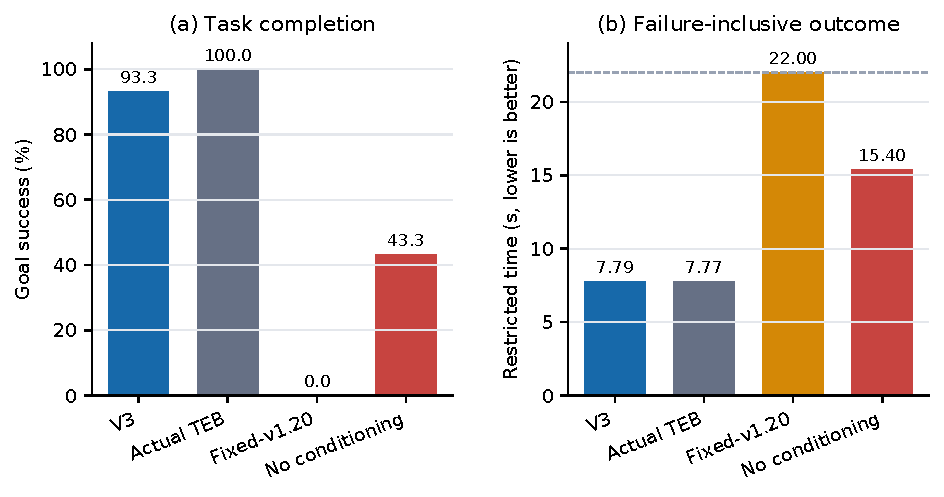
\includegraphics[width=0.98\textwidth]{figures/v3/fig01_method_outcomes.pdf}
\caption{V3-21 四方法成功率与失效计入式受限时间；失败以 22 s 保留。}
\label{fig:v321-outcomes}
\end{figure}

\section{配对效应与消融解释}
V3 与 Actual TEB 的受限均时分别为 7.785 s 和 7.770 s。配对相对降幅为 $-0.193\%$，双侧
95\% block-bootstrap 区间为 $[-19.867\%,12.982\%]$，Holm $p=0.755412$，因此该批 fresh
数据不支持 V3 的失效计入式时间优势。V3 相对 Fixed-v1.20 shielded 和去候选条件化消融则分别
缩短 64.614\% 与 49.454\%，两个 Holm $p$ 均为 0.000150。固定策略全部进入 certified stop，
只能说明该冻结直行策略过于保守，并不代表所有固定规划器。

\begin{table}[htbp]
\centering
\caption{V3-21 以配对区块为单位的比较结果。}
\label{tab:v321-comparisons}
\small
\begin{tabular}{lrrrr}
\toprule
比较对象 & 相对降幅/\% & 双侧95\% CI/\% & Holm $p$ & 成功率（V3/对方）\\
\midrule
Actual TEB 0.8.4 & -0.193 & [-19.867, 12.982] & 0.755412 & 93.3\%/100.0\%\\
Fixed-v1.20 shielded & 64.614 & [57.682, 69.250] & 0.000150 & 93.3\%/0.0\%\\
去候选条件化消融 & 49.454 & [37.001, 58.800] & 0.000150 & 93.3\%/43.3\%\\
\bottomrule
\end{tabular}
\end{table}


\begin{figure}[htbp]
\centering
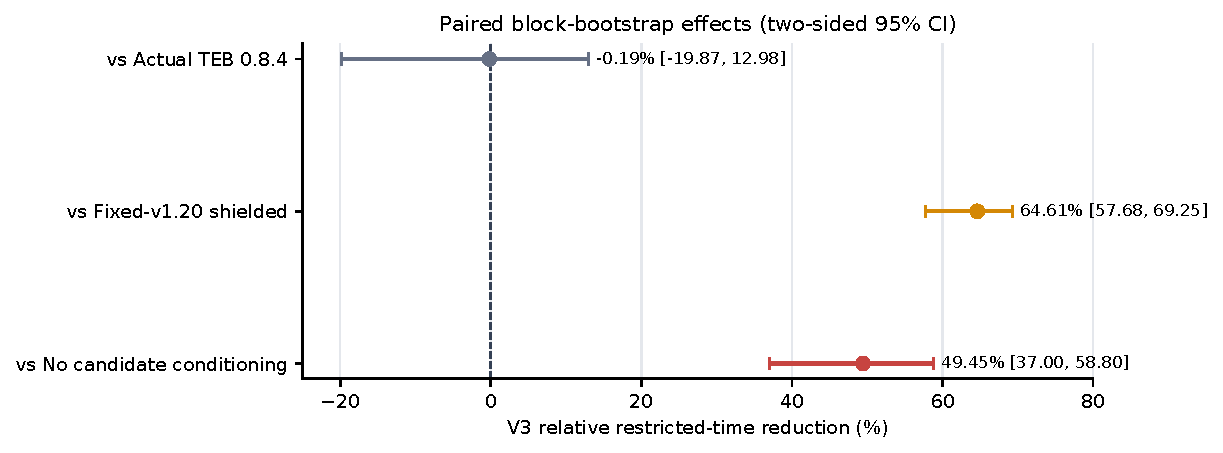
\includegraphics[width=0.95\textwidth]{figures/v3/fig02_pairwise_effects.pdf}
\caption{V3 相对三个比较对象的配对区块 bootstrap 效应；正值表示 V3 受限时间更短。}
\label{fig:v321-effects}
\end{figure}

\begin{figure}[htbp]
\centering
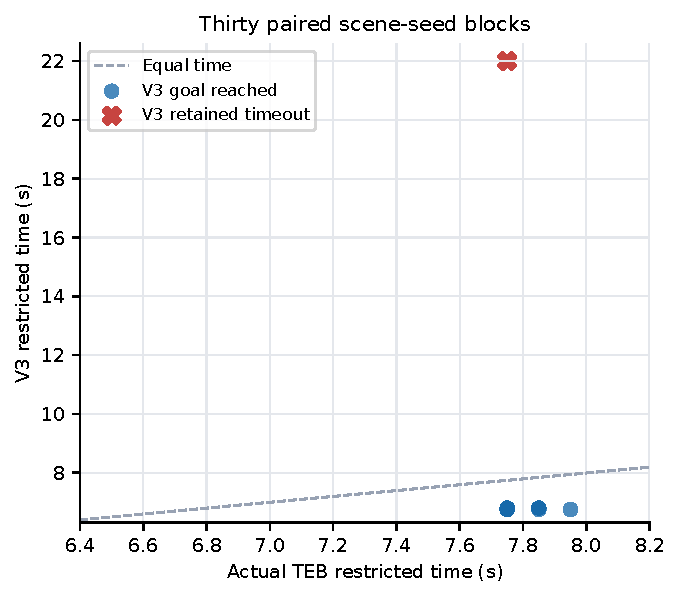
\includegraphics[width=0.67\textwidth]{figures/v3/fig03_v3_vs_actual_teb_blocks.pdf}
\caption{V3 与 Actual TEB 的 30 个配对区块；两个 V3 timeout 均保留为 22 s。}
\label{fig:v321-blocks}
\end{figure}

\section{分层、净空与协议偏差}
六个 scene$\times$policy strata 中，V3 在两个 hesitant strata 的成功率为 80\%，其余四层为
100\%；Actual TEB 六层均为 100\%。去候选条件化消融在 hesitant actor 下最弱，其中 open-90/
hesitant 为 0\%。这表明候选条件预测的探索性收益主要体现在避免保守停止，但不等价于相对
Actual TEB 的总体性能优势。

\begin{table}[htbp]
\centering
\caption{V3-21 六个场景--行为分层结果（成功率/受限均时）。}
\label{tab:v321-strata}
\scriptsize
\begin{tabular}{llrrrr}
\toprule
场景 & actor & V3 & Actual TEB & Fixed-v1.20 & 去条件化\\
\midrule
bounded-110 & cautious & 100\%/6.76s & 100\%/7.79s & 0\%/22.00s & 80\%/9.81s\\
bounded-110 & hesitant & 80\%/9.82s & 100\%/7.75s & 0\%/22.00s & 20\%/18.96s\\
open-90 & cautious & 100\%/6.76s & 100\%/7.75s & 0\%/22.00s & 60\%/12.86s\\
open-90 & hesitant & 80\%/9.82s & 100\%/7.81s & 0\%/22.00s & 0\%/22.00s\\
wide-70 & cautious & 100\%/6.77s & 100\%/7.75s & 0\%/22.00s & 60\%/12.87s\\
wide-70 & hesitant & 100\%/6.78s & 100\%/7.77s & 0\%/22.00s & 40\%/15.91s\\
\bottomrule
\end{tabular}
\end{table}


\begin{figure}[htbp]
\centering
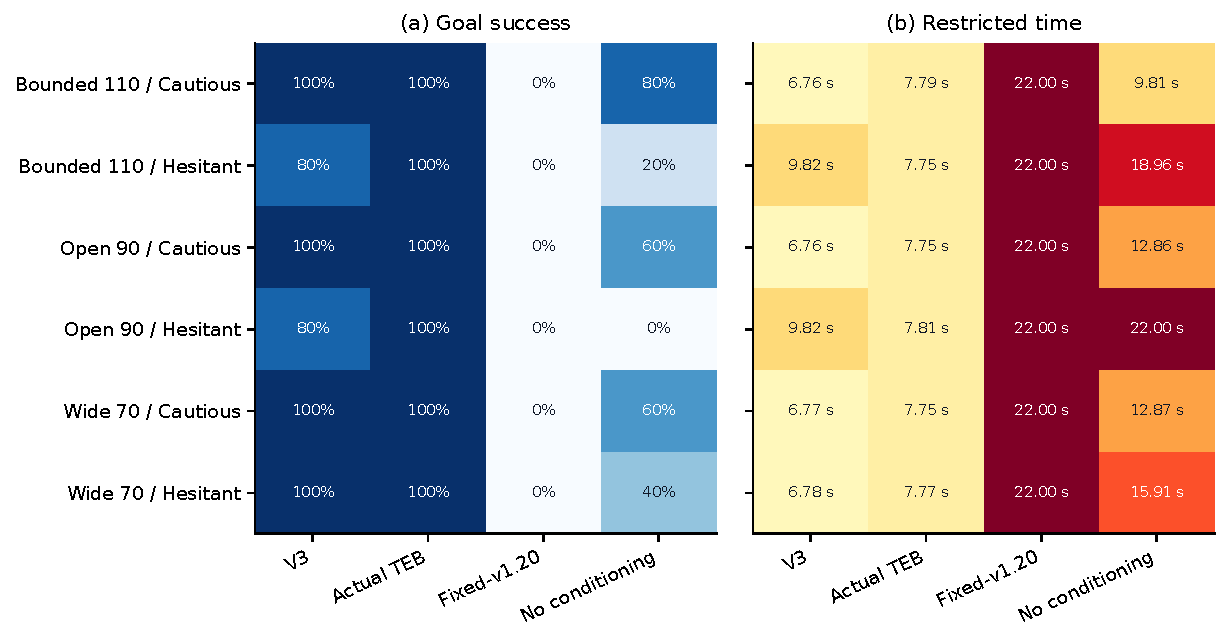
\includegraphics[width=0.98\textwidth]{figures/v3/fig04_scene_policy_strata.pdf}
\caption{六个冻结场景--actor 行为分层的成功率与受限时间。}
\label{fig:v321-strata}
\end{figure}

四方法 contact 均为 0；V3 与 Actual TEB 的最小经验净空分别为 0.4764 m 与 0.0395 m。图
\ref{fig:v321-clearance} 仅描述有限仿真样本，不构成形式化或实车安全结论。V3 规划延迟 P99 为
10.756 ms。唯一协议偏差出现在 sequence 107：gate x 误差 0.032286 m，超出 0.03 m 容差
2.286 mm；该回合目标成功且其余完整性门通过，故按 intention-to-treat 保留。排除对应 block 27
后的 V3--TEB 点降幅为 $-0.643\%$，结论不变。因存在该偏差，V3-21 的
\code{formal\_result=false}，但完整 120 回合表征和消融统计可报告。

\begin{figure}[htbp]
\centering
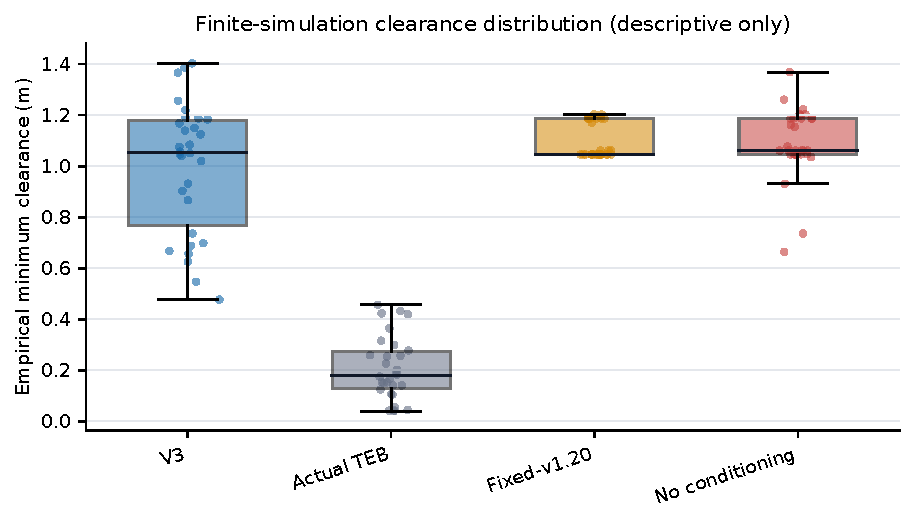
\includegraphics[width=0.94\textwidth]{figures/v3/fig05_minimum_clearance.pdf}
\caption{四方法经验最小净空分布；仅为有限仿真描述量。}
\label{fig:v321-clearance}
\end{figure}

\section{与历史正式阳性结果的关系}
V3-11 和 V3-21 使用不同 fresh seeds 与不同合同，必须分别报告。V3-11 双方均 30/30 成功，得到
12.9288\% 的正式阳性配对降幅；V3-21 将两个保守回退按 22 s 保留后不再优于 Actual TEB。
二者共同说明：成功通过时 V3 的完成时间稳定在约 6.77 s，但少量 certified-stop timeout 足以
消除失效计入式均值优势。论文因此保留 V3-11 的限定历史证据，同时明确陈述新的严格复现没有证明
Actual TEB 优势，不做事后合并、失败删除或选择性汇报。

\chapter{仿真特权信息驱动的候选轨迹强化学习}
\label{ch:pct-scope-rl}

\section{从 V3 解析规划到可部署强化学习}
V3-SCOPE 建立了“运动学可行候选---候选条件预测---硬验证---解析排序”的安全规划骨架，
但 V3-04 支持度审计表明，已有闭环日志对未执行候选的 propensity 为零，不能据此声称存在
可识别的 offline RL 收益。后续学习研究因此不修改 V3 冻结证据，而重新建立在线交互训练环境，
把强化学习权限限制在硬安全集合中的候选选择。

新系统称为 PCT-SCOPE-RL。它继承 V3 的候选级动作语义、解析先验、硬否决权和
certified-stop 思想，但使用独立的传感器 actor、训练合同和 fresh-seed 证据。部署端到端边界是
“真实可得传感器到候选轨迹 ID”，而不是“传感器到轮端控制量”。因此 V3 的 Gazebo 结果不能
被当作 V6 的学习结果，V6 的快速环境阳性也不能覆盖 V3 的 actual-TEB 证据边界。

\section{训练与部署架构}
\begin{figure}[htbp]
\centering
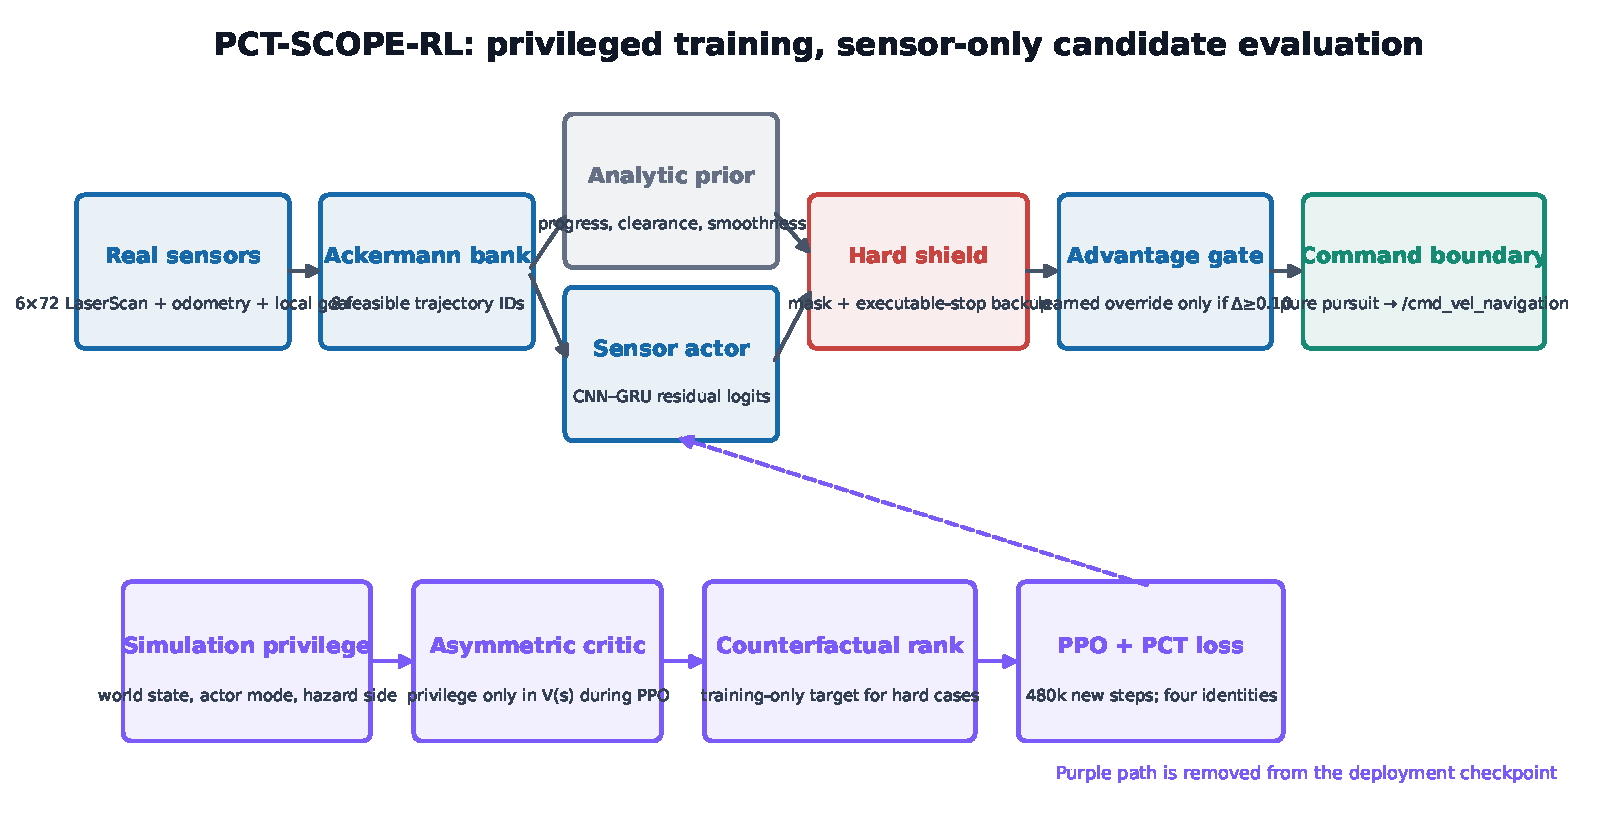
\includegraphics[width=\textwidth]{figures/v6/figure_v6_architecture.pdf}
\caption{PCT-SCOPE-RL 训练与部署数据流；紫色特权路径不进入 actor-only 部署检查点。}
\label{fig:v6-integrated-architecture}
\end{figure}

时刻 $t$ 的可部署观测为
\begin{equation}
o_t=(L_{t-5:t},\,v_t^{\mathrm{odom}},\,g_t,\,a_{t-1},\,v_{t-1}^{\mathrm{exec}}),
\end{equation}
其中 $L_{t-5:t}$ 是六帧、每帧 72 束的重采样激光历史，$g_t$ 是自车坐标系下的局部目标。
确定性运动学生成器产生 8 个候选：certified stop、三条直行速度候选以及四条左右空间候选。
每个候选附带目标速度、横向偏移、进度、净空、加速度、横向和平滑代价等描述。

解析先验 $q_{\mathrm{ana}}(o_t,\tau)$ 提供进度、净空和平滑性的基本排序。CNN--GRU actor
学习候选残差 $r_\theta(o_t,\tau)$，组合分数为
\begin{equation}
z_\theta(o_t,\tau)=\bar q_{\mathrm{ana}}(o_t,\tau)
+3\tanh r_\theta(o_t,\tau).
\end{equation}
硬验证器先产生掩码 $m_t$；被拒绝候选的 logit 被置为负无穷。只有当学习候选相对解析候选的
残差优势达到冻结阈值 0.10 时才允许覆盖，否则回退解析选择。最终候选由轨迹跟踪器转换到
\path{/cmd_vel_navigation}，原 GPS 限幅器、FOD 仲裁器和 M2 驱动安全边界保持在学习器之外。

\section{Asymmetric PPO 与 PCT 单因素}
主体策略通过 PPO rollout、GAE、裁剪策略目标、价值回归和熵正则学习
\cite{schulman2017ppo}。actor 只能编码 $o_t$，critic 额外读取 32 维仿真特权变量 $p_t$，包括
actor 世界位置、速度、模式、危险侧和候选未来净空：
\begin{equation}
L_{\mathrm{PPO}}=-L^{\mathrm{clip}}+c_vL_V-c_H\mathcal{H},
\qquad V_\phi=V_\phi(o_t,p_t).
\end{equation}
这一训练/部署信息分离与 asymmetric actor--critic 的一般思想一致
\cite{pinto2018asymmetric}，但 V5 正式实验表明，仅使用特权 critic 仍不足以达到预注册的
8\% 实效门。

V6 因此只增加 privileged counterfactual trajectory-rank distillation（PCT）。在部分遮挡和
窄走廊困难状态中，仿真危险侧与硬掩码构造候选排序目标 $a_t^\star(p_t,m_t)$；每次 PPO 更新后，
同一传感器 actor 接受一次权重为 0.35 的辅助交叉熵更新：
\begin{equation}
L_{\mathrm{V6}}=L_{\mathrm{PPO}}+\lambda_{\mathrm{PCT}}
\operatorname{CE}\!\left(\pi_\theta(\cdot\mid o_t,m_t),a_t^\star(p_t,m_t)\right),
\quad \lambda_{\mathrm{PCT}}=0.35.
\end{equation}
PCT 与 privileged teacher/student 方法相关\cite{chen2020cheating}，但它不训练独立的全状态驾驶
策略，而是把反事实候选排序蒸馏到仍由 PPO 回报优化的 actor 中。部署导出明确删除 critic、
特权编码器和 teacher target。

\section{训练链与正式实验设计}
V5 共执行 1,800,000 个训练环境步，形成 sensor-symmetric、asymmetric、no-prior 等冻结身份。
V5-03-F1 使用 60 个 fresh blocks，相对解析先验的失效计入受限均时降低 6.0936\%，双侧 95\%
区间为 [1.7867\%,11.0069\%]，但未达到预注册 8\% 最小实际效应，故是完整阴性结果。

离线归因后，V6 以四个 V5 检查点为初始化，使用新训练 seeds 9501--9504，各增加 120,000 步，
合计 480,000 步，无重试、扩展或额外因素轮次。验证 seeds 952100--952259 中四个身份方向均为正，
随后才释放 formal seeds 953100--953179。正式设计包含 80 个 Latin 分配区块和四种方法，共
320 个 episode；失败按 20 s 受限值计入，统计单位是 paired block。

\begin{figure}[htbp]
\centering
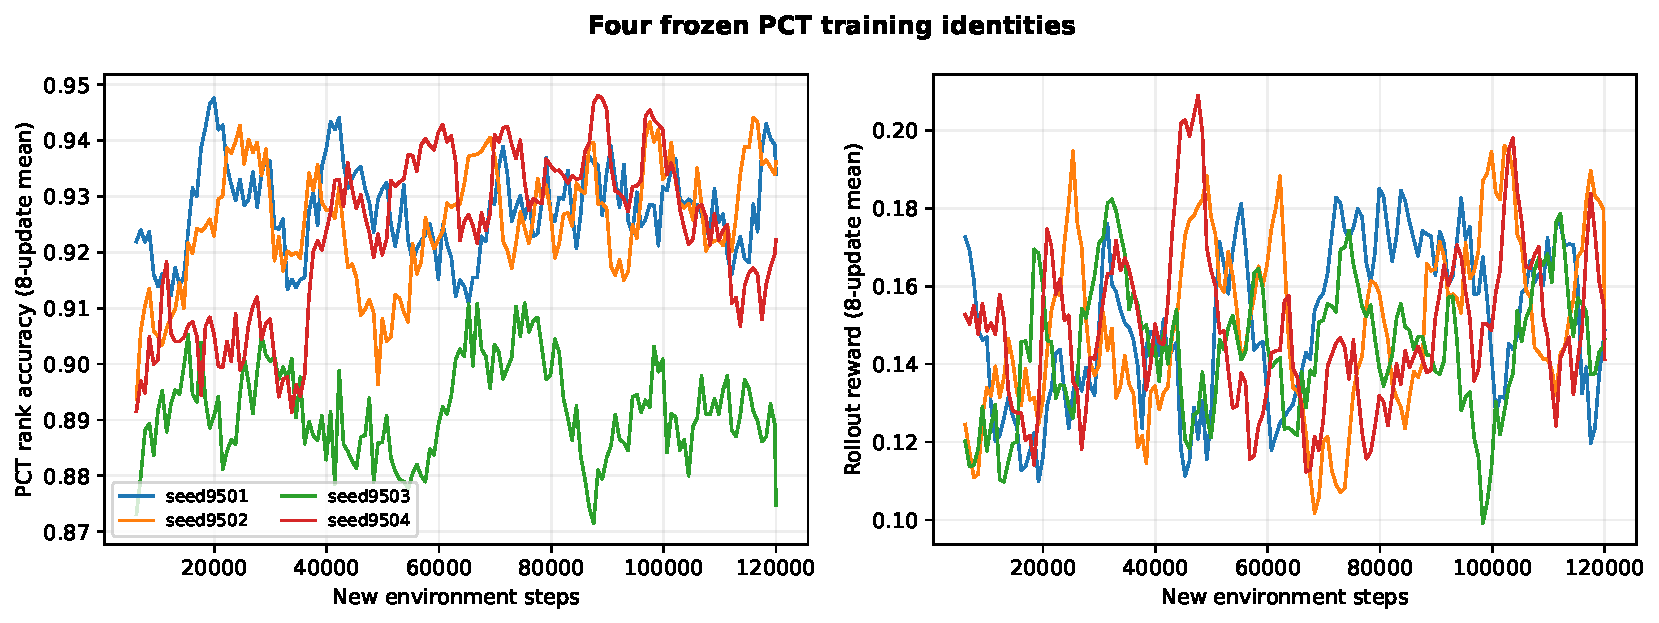
\includegraphics[width=.94\textwidth]{figures/v6/figure_v6_training.pdf}
\caption{四个 V6 训练身份的 PCT 候选排序准确率与 rollout reward。}
\label{fig:v6-integrated-training}
\end{figure}

\section{正式阳性结果与消融}
\begin{table}[htbp]
\centering
\caption{V6-02-F1 的方法级正式结果。}
\label{tab:v6-integrated-formal}
\begin{tabular}{lrrrrr}
\toprule
方法 & 回合 & 目标 & 受限均时/s & 最小净空/m & 接触/掩码违规\\
\midrule
解析先验 & 80 & 49 & 14.3188 & 0.1113 & 0/0\\
冻结 V5 & 80 & 56 & 13.5438 & 0.1055 & 0/0\\
PCT-SCOPE-RL V6 & 80 & 60 & 13.1156 & 0.1541 & 0/0\\
V6 no-history & 80 & 60 & 13.1156 & 0.1541 & 0/0\\
\bottomrule
\end{tabular}
\end{table}

\begin{figure}[htbp]
\centering
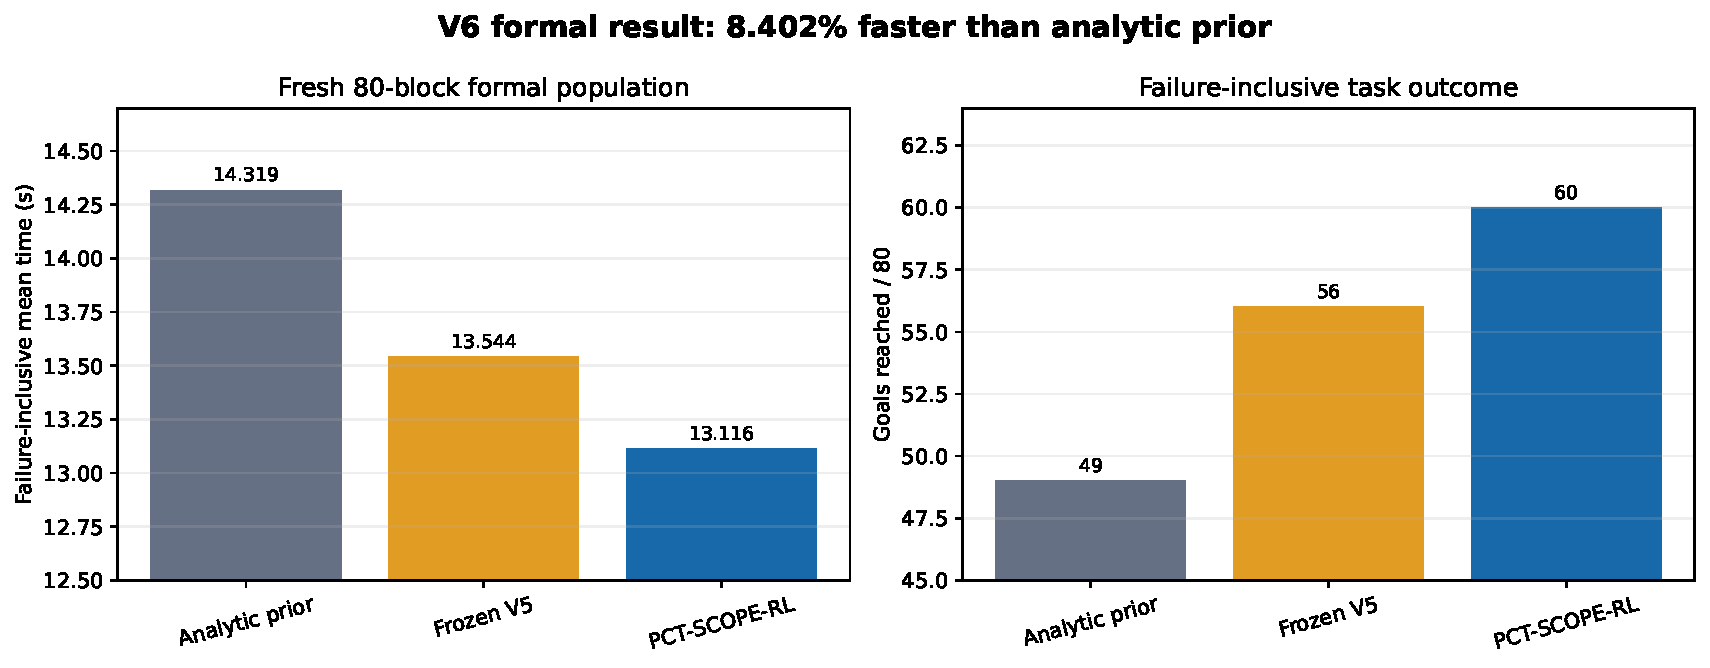
\includegraphics[width=.96\textwidth]{figures/v6/figure_v6_formal_summary.pdf}
\caption{80 个 fresh paired blocks 的方法均时和目标完成数。}
\label{fig:v6-integrated-formal}
\end{figure}

V6 相对解析先验的主效应为 8.4024\%，双侧 97.5\% block-bootstrap 区间为\\
$[3.4840\%,13.7135\%]$。点估计达到 8\% 门，区间下界严格为正，目标数不劣，接触与掩码违规
均为零，因此 \code{method\_effectiveness\_demonstrated=true}。相对冻结 V5 的次要降幅为
3.1611\%，双侧 95\% 区间为 [0.4936\%,6.5765\%]，支持 PCT 单因素产生附加收益。

\begin{figure}[htbp]
\centering
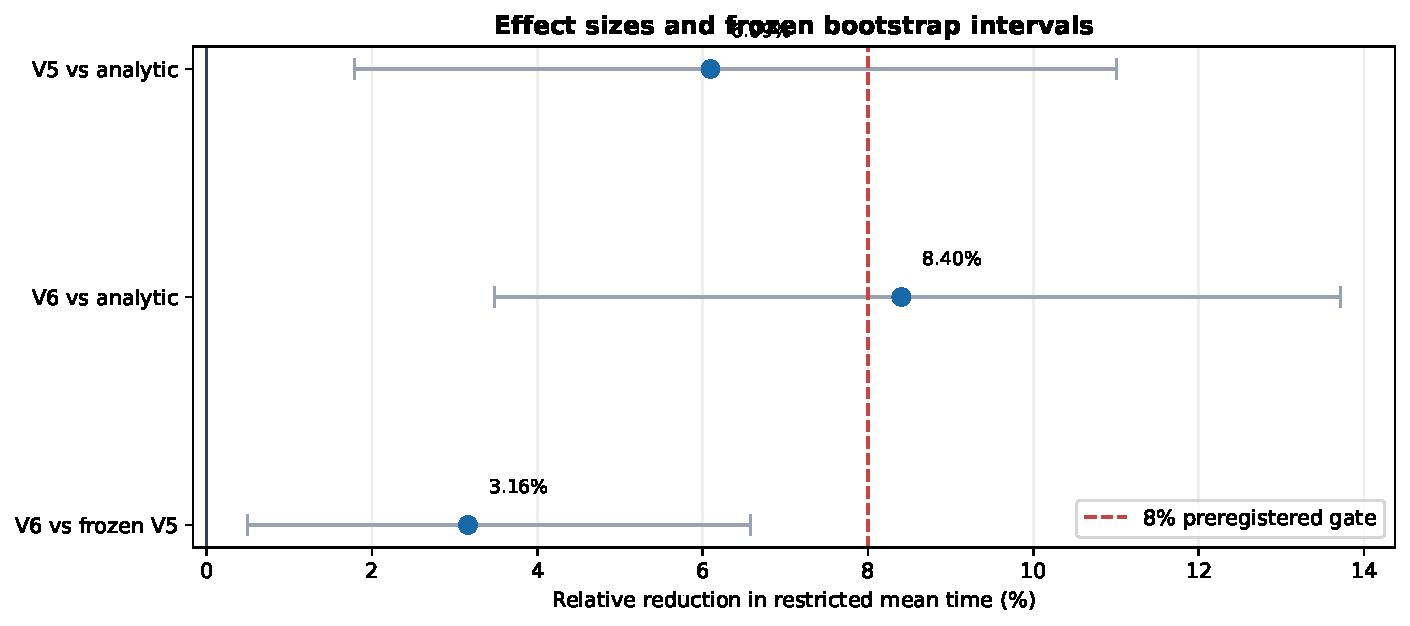
\includegraphics[width=.84\textwidth]{figures/v6/figure_v6_effect_intervals.pdf}
\caption{V5/V6 效应点估计与冻结 bootstrap 区间。}
\label{fig:v6-integrated-effects}
\end{figure}

\begin{figure}[htbp]
\centering
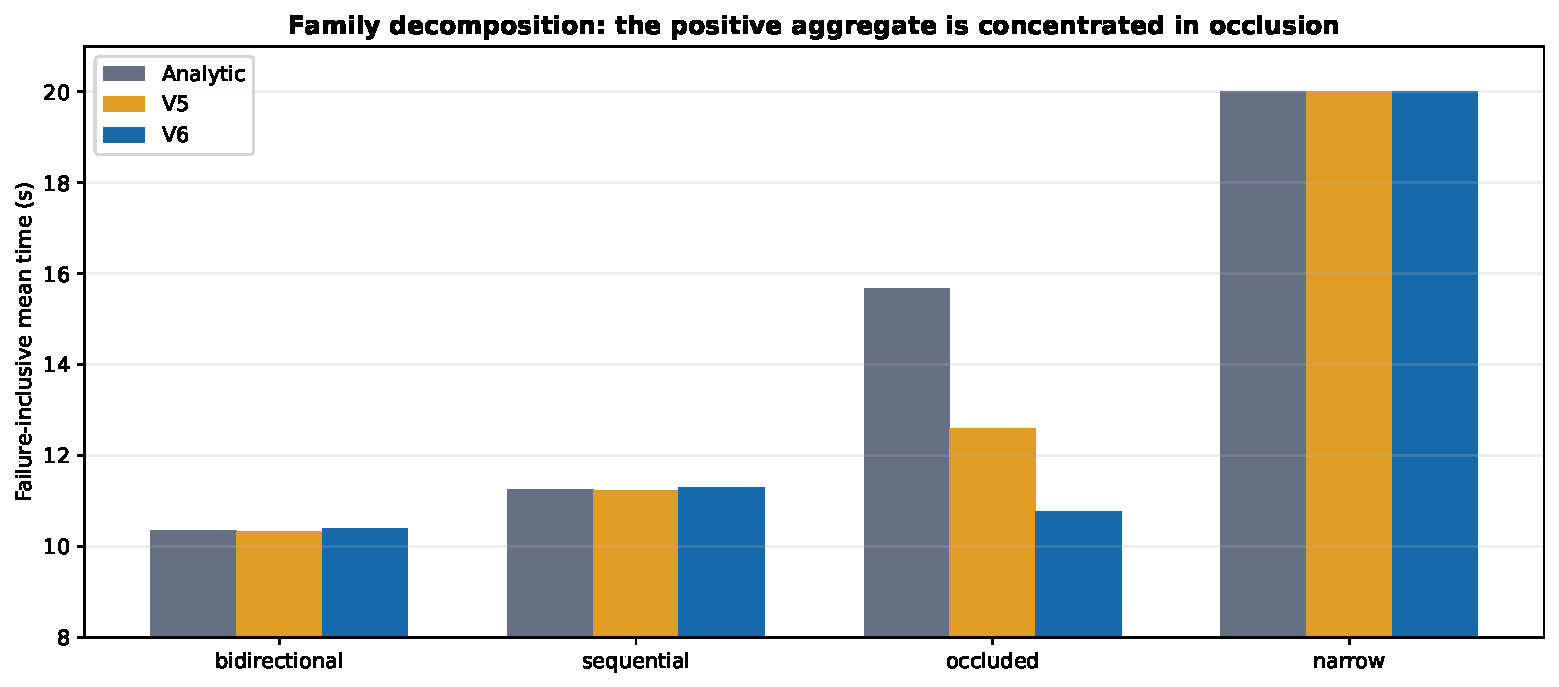
\includegraphics[width=.90\textwidth]{figures/v6/figure_v6_family_ablation.pdf}
\caption{四类交互总体的失效计入均时分解。}
\label{fig:v6-integrated-family}
\end{figure}

分场景结果显示，PCT 的主要收益来自部分遮挡 crossing：解析/V5/V6 受限均时分别为
15.675/12.600/10.7625 s，V6 完成 20/20，解析先验完成 9/20。窄走廊中三种方法均为
0/20，不能声称方法解决了一般让行问题。V6 与 no-history 的 80 个正式区块完全一致，故当前
证据不支持 GRU 历史记忆收益，阳性只能归因于冻结总体上的 PCT 候选偏好变化。

\section{Gazebo 迁移负结果}
\begin{figure}[htbp]
\centering
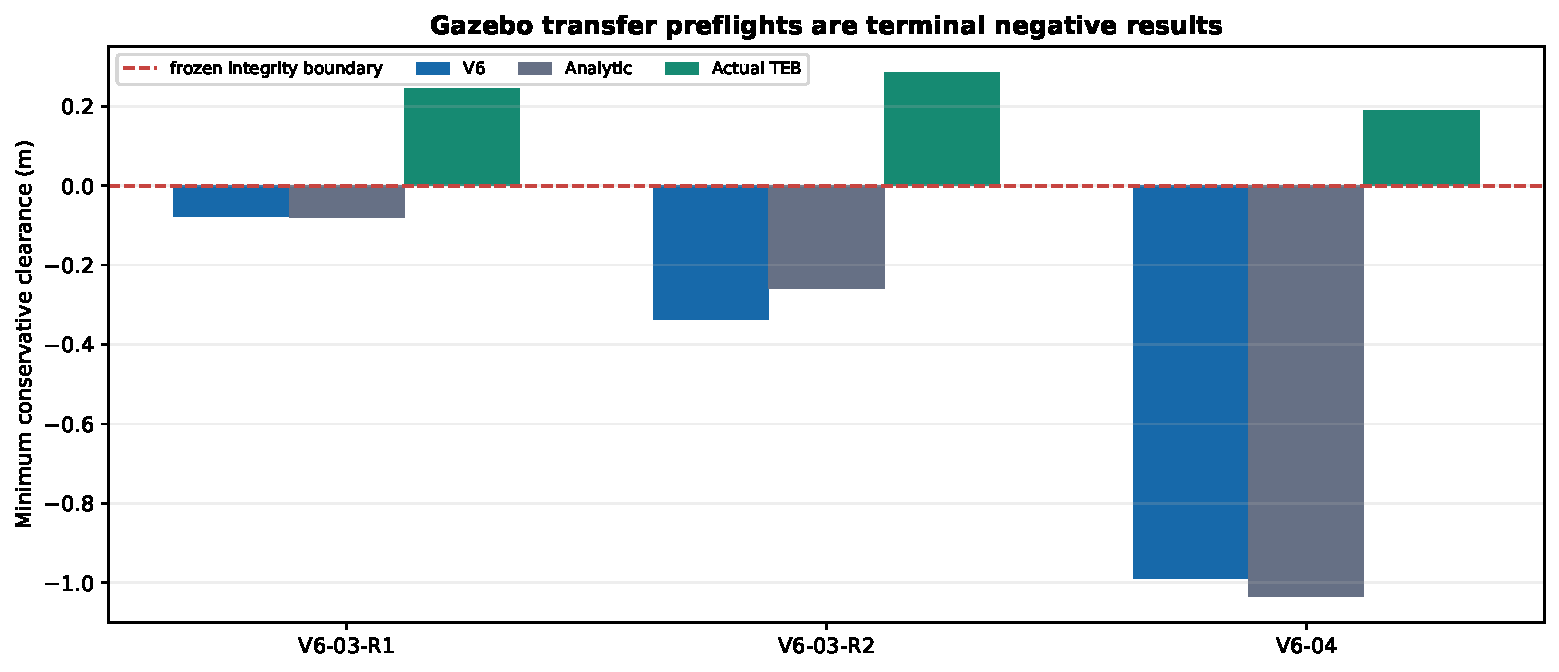
\includegraphics[width=.90\textwidth]{figures/v6/figure_v6_gazebo_boundary.pdf}
\caption{三次 Gazebo 迁移预检的最小保守净空；零线是冻结完整性门。}
\label{fig:v6-integrated-gazebo}
\end{figure}

三次新鲜单块预检中，V6/解析策略的保守净空分别为
$-0.077/-0.081$ m、$-0.337/-0.258$ m 和 $-0.990/-1.034$ m；Actual TEB 对应为
$+0.245/+0.285/+0.190$ m。最后一次预检中 V6 还发生 22 s timeout。虽然接触均为零，
冻结净空门已经失败，因此没有运行 Gazebo 资格或正式矩阵，也不存在 V6 相对 Actual TEB 的
有效性能比较。该结果不推翻快速总体内的阳性，但把外部有效性限制为：当前扫描屏蔽尚未形成
闭环交互一致的可达占据，不能声称 Gazebo、部署或实车有效。

\section{本章可支持的结论}
PCT-SCOPE-RL 的可辩护创新不是 PPO、privileged critic 或 shielding 中任一单项首创，而是
把“仿真特权候选排序蒸馏、部署期纯传感器候选评价、解析残差先验和硬否决权”组合为一个
action-aligned Ackermann 局部导航学习架构。正式证据支持冻结四类传感器级快速总体内的
8.4024\% 学习收益；不支持 temporal-history、Gazebo、一般 TEB 排名、形式化安全、感知/OOD、
多人泛化、部署或实车结论。



\chapter{实车实验设计与待补结果}
\label{ch:real-robot-placeholder}

\section{当前状态}
截至本文技术稿冻结时，尚未执行实车运动、CAN/串口访问、在线 TEB 参数写入或真实动态障碍测试。
本章仅保留学校最终论文所需的实验接口和表格结构，不提供、推测或插补任何实车数值。后续取得
现场条件和单独安全授权后，应以新的预注册研究填写本章；在此之前所有结果单元统一标记为
“待实车实验”。

\section{建议的分级验证流程}
\begin{enumerate}
  \item \textbf{传感器接口审计：}核对 LaserScan/点云、里程计、局部目标、TF、时间戳、视场、
  无回波语义和 72 束重采样，不允许运行时访问仿真特权字段。
  \item \textbf{静止 shadow：}机器人不运动，actor 只记录候选、优势门、硬掩码、certified-stop
  和推理延迟，不发布运动命令。
  \item \textbf{低速资格：}在封闭场地、物理急停、deadman、独立观察员和速度上限下，先静态障碍，
  再使用软质或遥控动态目标；资格阶段不得进入正式统计。
  \item \textbf{正式配对：}冻结 PCT-SCOPE-RL 与解析先验，按相同起终点和障碍行为随机化块内顺序，
  失败、急停和人工干预全部计入受限时间。
\end{enumerate}

\section{待填写的正式合同}
\begin{table}[htbp]
\centering
\caption{实车正式研究合同占位。}
\begin{tabularx}{\textwidth}{p{4.2cm}X}
\toprule
项目 & 冻结值\\
\midrule
车辆、传感器与计算平台 & 待实车实验\\
场地与场景数量 & 待实车实验\\
比较方法 & 建议：解析先验、冻结 V6；Actual TEB 作为可选次要基线\\
正式 paired blocks & 待功效分析后冻结\\
主要指标 & 失败计入受限完成时间\\
安全门 & 零接触、零未计划急停、独立最小净空达到预注册阈值\\
外部真值 & 待定；只能用于评价，不得进入 actor\\
排除、停止和失败计入规则 & 待预注册\\
\bottomrule
\end{tabularx}
\end{table}

\section{待填写的结果表}
\begin{table}[htbp]
\centering
\caption{实车结果占位；不得在没有原始日志时填写。}
\begin{tabular}{lrrrrr}
\toprule
方法 & 回合 & 目标成功 & 受限均时/s & 最小净空/m & 接触/干预\\
\midrule
解析先验 & -- & -- & -- & -- & --\\
PCT-SCOPE-RL V6 & -- & -- & -- & -- & --\\
Actual TEB（可选） & -- & -- & -- & -- & --\\
\bottomrule
\end{tabular}
\end{table}

\section{允许的占位结论}
在实车证据产生之前，本章唯一允许的结论是：“实车评估尚未执行，当前论文结论来自限定仿真总体；
实车实验是后续外部有效性验证，而不是已经完成的证据。”



\chapter{讨论}
\section{V3 安全骨架与 V6 学习层的关系}
V3 与 V6 共享候选级动作、硬否决权和解析回退的研究范式，但它们使用独立实现、种子与证据。V3 解决候选条件预测和可行空间选择，V6 解决仿真特权如何通过 PCT 改善部署期纯传感器候选评价。两者构成递进架构，不允许把 V3 的 Gazebo 阳性移植为 V6 的学习或感知证据。

\section{内部阳性与迁移阴性为何可以并存}
V6-02-F1 回答冻结快速交互总体中的学习收益，V6-03/04 则检查扫描、跟踪、占据和跟踪器组成的Gazebo 闭环迁移链。前者通过说明 PCT 在该总体内有效；后者失败说明当前感知--verifier 接口不能承载同样的外部结论。二者不是统计矛盾，而是内部有效性与外部有效性的不同层级。

\section{历史阳性与新鲜未复现为何可以并存}
历史 V3-11 回答冻结正式合同下的配对性能问题，V3-21 则加入固定比较与单因素消融，并要求失败全部
进入 22 s 统计。新实验不是对旧证据的删除，但降低了“稳定优于 Actual TEB”这一更强陈述的可信度。
工程上最重要的限制是硬安全验证可能选择 certified stop：它提高了保守性，却使任务效率对少量
拒绝事件高度敏感。后续研究应在不放松安全门的前提下改进可行候选覆盖，而不是删除失败区块。

\section{为什么单演员阳性与多人阴性可以同时成立}
V3-11 检验的是冻结单演员总体上的规划器时间收益；V3-14/V3-16 检验的是在两个闭环 actor 下，不同候选
是否共享足够一致的分支前状态，以支持 cloned-intervention predictor 拟合。二者研究问题、seed、
合同与资格门不同。单演员规划收益成立，并不逻辑蕴含多人反事实可比性成立。

\section{工程意义}
动作绑定闭环消除了“调度动作不等于运行动作”的证据风险。更重要的是，V3-14/V3-16 显示完整性修复不应
自动升级科学结论：执行器可以完美执行错误或不可比的实验。将 runtime identity、反事实配对和性能
推断拆成不同 gate，是本项目对可复现实验流程的关键贡献。

\section{有效性威胁}
\begin{itemize}
  \item 场景是工程构造的 Gazebo 模板，actor policy 不是实测人群分布；
  \item actual TEB 比较只覆盖 0.8.4 与冻结配置，不是所有版本/调参的排序；
  \item oracle actor track 隔离了规划器差异，也排除了感知误差，故不能声明感知鲁棒；
  \item 零 contact 和保守净空是有限仿真总体上的经验量，不是形式化安全证明；
  \item 没有实车、定位漂移、传感器退化、复杂静态地图或多人正式性能证据；
  \item V3 的训练步数为 0，不能声称 V3 学习收益；V6 另建在线交互训练并取得限定快速总体阳性，但 Gazebo 迁移失败。
  \item V3-21 有一个超出 gate 容差 2.286 mm 的协议偏差，故只能作完整表征；排除敏感性虽不改变
  结论，也不能把它事后升级为正式研究。
\end{itemize}

\chapter{结论与展望}
本文形成了从高维参数动作诊断、解析安全候选规划到仿真特权强化学习的完整研究链。T12/V2
揭示 commanded parameter 与 executed action 的投影错位；V3-SCOPE 以 Ackermann 可行轨迹、
候选条件预测、校准占据、硬验证和解析排序建立 action-aligned 骨架。V3-11 提供了限定单 actor
Gazebo 总体中的历史 actual-TEB 阳性证据，而 V3-21 在保留 timeout 的新鲜四方法研究中没有复现
普遍优势，说明候选条件机制存在，但少量保守停止足以消除 failure-inclusive 时间收益。

在 V3 骨架基础上，PCT-SCOPE-RL 把强化学习权限限制为安全候选集合中的轨迹 ID 选择。actor
部署时只读取真实可得传感器，仿真特权只用于 asymmetric critic 和 PCT 候选排序目标；解析先验、
优势门和硬屏蔽限制学习覆盖。V5 未达到 8\% 实效门后，V6 只增加 PCT 单因素，并在 80 个 fresh
paired blocks 上得到 8.4024\% 主效应和严格为正的双侧 97.5\% 区间，且相对 V5 仍有 3.1611\%
附加收益。这构成本文的核心强化学习阳性结论。

结论必须保持范围限定：收益集中在部分遮挡总体，窄走廊未解决，no-history 消融完全相同；三次
Gazebo 传感器迁移预检又均未通过保守净空门。因此当前工作证明的是冻结传感器级快速总体内的
特权候选排序蒸馏收益，而不是一般动态导航、形式化安全、Actual TEB 排名、部署或实车有效性。
后续应首先建立闭环交互一致的传感器占据与验证链，再通过 shadow、低速资格和预注册配对矩阵补充
实车外部有效性；在真实数据产生之前，本文实车章节保持为空。

\appendix
\chapter{主要冻结证据索引}
\begin{longtable}{p{0.31\textwidth}p{0.62\textwidth}}
\toprule
资产 & SHA-256\\
\midrule
\endhead
V3-11 formal assessment & \hashbreak{9b19f8bd29f1d6c0}{6197e932b03359a2}{f78081da65e636f5}{2f7f610529c3f2f9}\\
V3-11 independent review & \hashbreak{2d5e8c21ea70f29d}{f97e646f70315929}{7ff0d2da6ef10edb}{1341da057c133b39}\\
V3-12 paper manifest & \hashbreak{319bce3401859e25}{fa1e5da68d97669a}{6aebf593688c4750}{03a8844b91798c0b}\\
V3-14 execution release & \hashbreak{bf2cf4ec95861897}{5597ce46f6f150d4}{279d68d7548e7dfa}{c39e08333943855a}\\
V3-14 evidence summary & \hashbreak{d6ffde4c658170cc}{f6ed992bd4131ee2}{8f72a81882d64f73}{b41c38038f53e8d4}\\
V3-14 assessment & \hashbreak{58c472560699e102}{76f76c063dd243ab}{5666f8e534346c51}{e88aa9f2b49958b9}\\
V3-14 evidence manifest & \hashbreak{ab8d31605b383a7b}{590f86f716a6fe88}{a2eb12c2afb45f74}{e21195a7f47b4679}\\
V3-14 independent review & \hashbreak{4773d76437a01148}{984770ca502dce96}{cfa6d3bc2743029e}{0bb7a1f10f94c60a}\\
V3-16-D1 attribution & \hashbreak{1f84987b14a9a872}{1eea5823e965d7c0}{283f0a4250f7efb7}{137cf060b08e7396}\\
V3-16 execution release & \hashbreak{8bdb5eebebaf1cde}{d5b2712fd51d92cc}{e134858255f7f877}{6cfb1f7076618a71}\\
V3-16 evidence summary & \hashbreak{088483a89952f157}{b51f5411a96e270f}{3d639c214a244d1d}{6fbdbc4b9e116590}\\
V3-16 R1 assessment & \hashbreak{6a30f54abea88949}{722cf10e58e4da59}{aaa11a631f9eece2}{ee373a9f766ebaf5}\\
V3-16 R1 review & \hashbreak{c4469571a1a8f8e9}{99e733138d42466f}{a0c0a6bd472bcebe}{5d044fe512a4765c}\\
V3-21 characterization & \hashbreak{c195fc7cea4c6495}{82bb3c0017e55a1b}{98f5de3b7f971737}{b1f2abcb5596ccc8}\\
V3-21 independent review & \hashbreak{450f4103e58e8e62}{2c3adc192599a6e7}{4fdc587430277432}{a642403729e6dd90}\\
V3-22 paper materials manifest & \hashbreak{658e906c3fae23d8}{6e5cab5e65edbe6c}{a00cc74c1188b040}{4294f29c4fe973d0}\\
V3-22 paper materials review & \hashbreak{88547275a6627027}{517aa55d2128469b}{b30de1721fc162e9}{2ab9d6d787be0959}\\
V5 formal assessment & \hashbreak{683d2823db46179c}{44633c70210e47ec}{7cf0df3a6ed3e8e5}{ec8bd70a0da59e25}\\
V6 formal assessment & \hashbreak{08a0ab06343cad51}{ee206ba502d2a115}{c6fd707d58620f9b}{b4f519a71ec95c1b}\\
V6 paper review & \hashbreak{ff4b6423d8fb610f}{e29486ab059c86a1}{e86f284055c8b520}{cf9e38cf4e470b41}\\
\bottomrule
\end{longtable}

\chapter{论文声明门}
\begin{longtable}{p{0.18\textwidth}p{0.22\textwidth}p{0.52\textwidth}}
\toprule
声明 & 状态 & 合法边界\\
\midrule
\endhead
历史单演员 actual TEB 时间收益 & qualified historical & V3-11 的三个冻结模板、固定 TEB 0.8.4 配置、共享 oracle track。\\
新鲜失效计入式 TEB 优势 & not demonstrated & V3-21 点降幅 $-0.193\%$，双侧 95\% CI 跨零；不得与 V3-11 合并。\\
候选条件化消融机制 & exploratory evidence & V3-21 相对去条件化消融降幅 49.454\%，成功率 93.33\%/43.33\%。\\
多人五动作支持 & not demonstrated & V3-16 速度门通过但坐标门仍失败；不得拟合 predictor。\\
响应门控因素 & qualified mechanism & 速度最大差下降 88.07\%；不等于整体共同前缀或性能通过。\\
V5 特权 critic 学习收益 & not demonstrated & 6.0936\% 未达到预注册 8\% 实效门。\\
V6 PCT 快速总体收益 & qualified & 8.4024\%，双侧 97.5\% CI [3.4840\%,13.7135\%]；仅限四类冻结 sensor-level fast population。\\
V6 Gazebo/Actual TEB 收益 & not demonstrated & 三次预检净空门失败，资格和正式矩阵均未运行。\\
时序历史收益 & not demonstrated & V6 与 no-history 在 80 个正式块上完全相同。\\
感知/OOD 泛化 & forbidden & 未运行感知退化或 OOD 正式研究。\\
形式化安全 & forbidden & 当前仅有限仿真经验门。\\
V3 学习收益 & forbidden & V3 训练步数为 0；V6 是独立训练和证据链。\\
实车与部署 & pending/not demonstrated & 当前无硬件执行；实车章节只保留待补合同和空表。\\
\bottomrule
\end{longtable}

\begin{thebibliography}{9}
\bibitem{schulman2017ppo} J. Schulman et al., ``Proximal Policy Optimization Algorithms,'' arXiv:1707.06347, 2017.
\bibitem{pinto2018asymmetric} L. Pinto et al., ``Asymmetric Actor Critic for Image-Based Robot Learning,'' RSS, 2018.
\bibitem{chen2020cheating} D. Chen et al., ``Learning by Cheating,'' CoRL, PMLR 100, 2020.
\bibitem{alshiekh2018shielding} M. Alshiekh et al., ``Safe Reinforcement Learning via Shielding,'' AAAI, 2018.
\bibitem{carr2022partialshield} S. Carr et al., ``Safe Reinforcement Learning via Shielding under Partial Observability,'' 2022.
\bibitem{rosmann2017teb} C. Rösmann, F. Hoffmann, and T. Bertram, ``Integrated Online Trajectory Planning and Optimization in Distinctive Topologies,'' Robotics and Autonomous Systems, 2017.
\bibitem{long2017sensorrl} P. Long et al., ``Towards Optimally Decentralized Multi-Robot Collision Avoidance via Deep Reinforcement Learning,'' 2017.
\end{thebibliography}

\end{document}
